%%# -*- coding:utf-8 -*-

\documentclass{article}
% if you need to pass options to natbib, use, e.g.:
%     \PassOptionsToPackage{numbers, compress}{natbib}
% before loading neurips_2022


% ready for submission
% \usepackage{neurips_2022}


% to compile a preprint version, e.g., for submission to arXiv, add add the
% [preprint] option:
%     \usepackage[preprint]{neurips_2022}

\PassOptionsToPackage{numbers, compress}{natbib}  % ref https://arxiv.org/abs/2209.09407
% to compile a camera-ready version, add the [final] option, e.g.:
\usepackage[final]{neurips_2022}

% to avoid loading the natbib package, add option nonatbib:
%    \usepackage[nonatbib]{neurips_2022}

% \usepackage[utf8]{inputenc} % allow utf-8 input
\usepackage[T1]{fontenc}    % use 8-bit T1 fonts
\usepackage{hyperref}       % hyperlinks
\usepackage{url}            % simple URL typesetting
\usepackage{booktabs}       % professional-quality tables
\usepackage{amsfonts}       % blackboard math symbols
\usepackage{nicefrac}       % compact symbols for 1/2, etc.
\usepackage{microtype}      % microtypography
\usepackage{xcolor}         % colors
\usepackage{graphicx}       %%  图片包
\usepackage{subfig}
\usepackage{geometry}
\usepackage{calligra}
\usepackage{algorithm}
\usepackage{algorithmicx}
\usepackage{algpseudocode} 
\usepackage{amsmath}
\usepackage{amssymb}
\usepackage{bm}
\usepackage{multirow}
\usepackage{diagbox}
\newtheorem{definition}{Definition}[section]
\newtheorem{theorem}{Theorem}[section]
\newtheorem{notations}{Notations}

\title{Reproduction of ``Fast and Accurate Matrix Completion via Truncated Nuclear Norm Regularization''}


% The \author macro works with any number of authors. There are two commands
% used to separate the names and addresses of multiple authors: \And and \AND.
%
% Using \And between authors leaves it to LaTeX to determine where to break the
% lines. Using \AND forces a line break at that point. So, if LaTeX puts 3 of 4
% authors names on the first line, and the last on the second line, try using
% \AND instead of \And before the third author name.


\author{%
  Zhao-Yang Liu\\ %\thanks{Use footnote for providing further information
    % about author (webpage, alternative address)---\emph{not} for acknowledging
    % funding agencies.} \\
    Sun Yat-sen University \\
  \texttt{liuzhy86@mail2.sysu.edu.cn} \\
  % examples of more authors
  \and
  Xin-Hua Zheng \\
  Sun Yat-sen University \\
  \texttt{zhengxh56@mail2.sysu.edu.cn} \\
  % \AND
  % Coauthor \\
  % Affiliation \\
  % Address \\
  % \texttt{email} \\
  % \And
  % Coauthor \\
  % Affiliation \\
  % Address \\
  % \texttt{email} \\
  % \And
  % Coauthor \\
  % Affiliation \\
  % Address \\
  % \texttt{email} \\
}


\begin{document}
{

\maketitle

\begin{abstract}
Recovering a large matrix from a small subset of its entries is a challenging problem arising in many real applications, such as computer vision. This can be considered as a low rank matrix approximation problem. If the nuclear norm is used as a convex relaxation of the rank operator, all singular values are minimized simultaneously by minimizing the nuclear norm, so the rank is not well approximated in practice. 
Hu proposed to achieve a better approximation to the rank of matrix by truncated nuclear norm, which is given by the nuclear norm subtracted by the sum of the largest few singular values. Furthermore, they developed a novel matrix completion algorithm and further developed three efficient iterative procedures TNNR-ADMM, TNNR-APGL and TNNR-ADMMAP to solve the optimization problem.
In this report, we reproduce the algorithm of Hu et al. and related work, and perform experiments similar to their work. Our experiments show encouraging results of the algorithm proposed by Hu et al. in comparison to the related work on both synthetic and real visual datasets.
\end{abstract}


\section{Introduction}
For the problem of estimating missing values in a matrix, or matrix completion, a commonly adoped assumption is the underlying matrix has a low rank or approximately low rank structure.
The visual data, such as images, is probably of low rank structure, as shown in Fig.~\ref{fig1}.
Specifically, given the incomplete data matrix $\mathbf M \in \mathbb{R}^{m \times n}$ of low rank, the matrix completion problem can be formulated as follows:
\begin{equation}
    \begin{aligned}
        \min_{\mathbf X}\qquad&\quad \text{rank}(\mathbf X) \\
        \text{s.t.}\qquad&\quad\mathbf X_{ij} =\mathbf M_{ij}, \ (i,j) \in\mathbf \Omega,
    \end{aligned}
    \label{rmin}
\end{equation}
where $\mathbf X \in \mathbb{R}^{m \times n}$ and $\mathbf \Omega$ is the set of locations corresponding to the observed entries.

Unfortunately, the rank minimization problem is NP-hard in general and is also NP-hard to approximation.  A widely used approach is to apply the nuclear norm (i.e., the sum of singular values) as a convex surrogate for the rank function of a non-convex matrix. It has been shown that under some general constraints, nuclear norm minimization can recover incomplete matrices from enough observed entries.

In this report, we reproduce a matrix completion algorithm called truncated nuclear norm regularization (TNNR) and three optimization schemes proposed by Hu et al\cite{hu.he201309}: the alternating direction method of multipliers (ADMM), the accelerated proximal gradient line search method (APGL) and the Alternating Direction Method of Multipliers with Adaptive Penalty (ADMMAP). 
Unlike other nuclear norm methods, TNNR only minimize the smallest $\min(m, n) - r$  singular values since the rank of a matrix only corresponds to the r non-zero singular values. 

In Section~\ref{s2}, we briefly introduce three kinds of work related to matrix completion. In Section~\ref{s3}, we introduce the TNNR algorithm and three optimization schemes. In Section~\ref{s4}, we conduct experiments similar to the original paper and give the experimental results. In Section~\ref{s5}, we summarize what we have accomplished.

\begin{figure}[htbp]
    \centering
    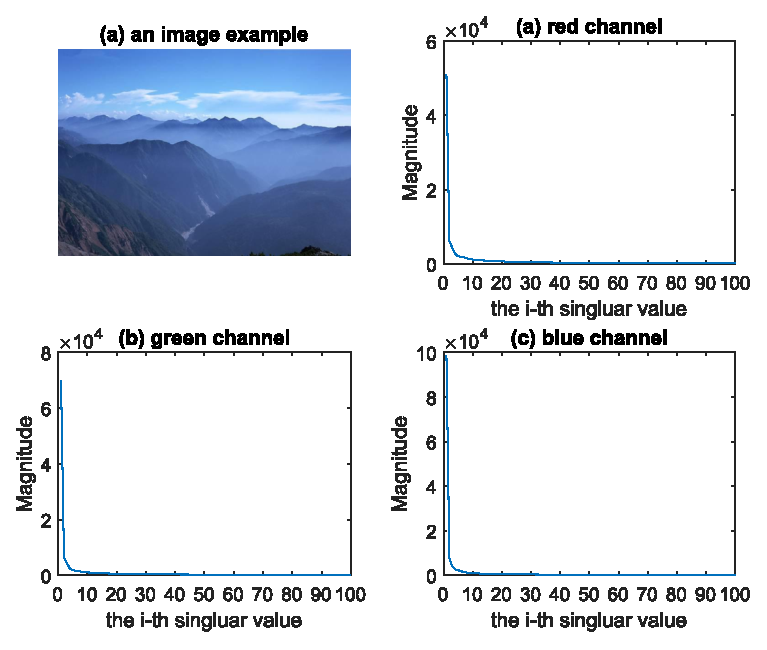
\includegraphics[width=0.6\textwidth]{assets/fig1.eps}
    \caption{A 400 $\times$ 500 image example}
    \label{fig1}
\end{figure}

\begin{notations}
    Let $\mathbf X = (\mathbf x_1,\cdots,\mathbf x_n)$ be an $m \times n$ matrix, $\mathbf \Omega \in \{1,\cdots,m\}\times\{1,\cdots,n\}$ denote the indices of the observed
    entries of $\mathbf X$, and let $\mathbf \Omega_c$denote the indices of the missing entries. The Forbenius norm of $\mathbf X$ is defined as $\lVert\mathbf X \rVert_F = \sqrt{\sum_{(i,j)} \mathbf X^2_{i,j}}$. Let $\mathbf X=\mathbf U\mathbf \varSigma \mathbf V^T$ be the singular value decomposition for $\mathbf X$, where $\varSigma = diag(\sigma_i)$, $1 \leq i\leq \min\{m,n\}$, and $\sigma_i$ is the ith largest singular value of $\mathbf X$. The nuclear norm of $\mathbf X$ is denoted as $\lVert\mathbf X \rVert_* = \sum_{i=1}^{\min(m,n)} \sigma_i$ . Let $\mathcal{P}_{\mathbf \Omega}$ be the orthogonal projection operator onto the span of matrices vanishing outside of $\mathbf \Omega$ so that
    \begin{equation*}
        (\mathcal{P}_{\mathbf \Omega}(\mathbf X))_{ij} = \begin{cases}
            \mathbf X_{ij} & \text{\rm if } (i,j) \in \mathbf \Omega\\
        0 & \text{\rm if } (i,j) \in \mathbf \Omega^c
    \end{cases}
    \end{equation*}
    The  inner product of the matrix space is defined as $ \langle \mathbf X,\mathbf Y\rangle = \sum_{i,j} = \mathbf X_{ij}\mathbf Y_{ij}$.
\end{notations}

\begin{definition}
    Consider the SVD of a matrix $\mathbf X \in \mathbb{R}^{m \times n}$:
    \begin{equation}
        \mathbf X = \mathbf U \mathbf \varSigma \mathbf V^T, \ \mathbf \varSigma = diag(\{\sigma_i\}_{1 \leq \min(m,n)}).
    \end{equation}
    Define the singular value shrinkage operator $D_{\tau}$ as follows:
    \begin{equation}
        D_{\tau}(\mathbf X) = \mathbf U D_{\tau}(\mathbf \varSigma) \mathbf V^T, \ D_{\tau}(\mathbf \varSigma) = diag(\max\{\sigma_i-\tau,0\}).
    \end{equation}
    We have the following useful theorem:	
\end{definition}

\begin{theorem}
    For each $\tau \geq 0$ and $\mathbf Y \in \mathbb{R}^{m \times n}$, we have
    \begin{equation}
        D_{\tau}(\mathbf X) = \underset{\mathbf X}{\arg\min}\  \frac{1}{2} \lVert \mathbf X-\mathbf Y\rVert_F^2 + \tau \lVert\mathbf X \lVert_*.
    \end{equation} 
    \label{thm32}
\end{theorem}

\section{Related work}
\label{s2}


In this section, we introduce three methods for matrix completion: singular value thresholding (SVT)\cite{cai.shen200810},  singular value projection (SVP)\cite{jain.dhillon2010}, and Optspace\cite{keshavan.montanari200906}. These methods are also used to compare with the TNNR algorithm in subsequent experiments. In addition, ADMM and APDL is is briefly explained for better algorithm derivation in Section~\ref{s3}.

By approximating the rank function using the nuclear norm to solve the rank
minimization problem~\eqref{rmin},  the matrix completion problem can be formulated as follows:
\begin{equation}
    \begin{aligned}
        \min_{\mathbf X}\qquad&\quad \lVert\mathbf X\rVert_* \\
        \text{s.t.}\qquad&\quad  \mathcal{P}_{\mathbf \Omega}(\mathbf X) =  \mathcal{P}_{\mathbf\Omega}(\mathbf M).
    \end{aligned}
    \label{normf}
\end{equation}

For SVT, Cai et al. propose the SVT algorithm :
\begin{equation}
    \begin{aligned}
        \min_{\mathbf X}\qquad&\quad \lVert\mathbf X\rVert_* + \alpha\lVert \mathbf X\rVert_F^2\\
        \text{s.t.}\qquad&\quad\mathcal{P}_{\mathbf\Omega}(\mathbf X) =  \mathcal{P}_{\mathbf\Omega}(\mathbf M).
    \end{aligned}
\end{equation}
Construct the Lagrangian function,
\begin{equation}
    \mathcal{L}(\mathbf X,\mathbf Y) = \lVert\mathbf X\rVert_* + \alpha\lVert \mathbf X\rVert_F^2 + \langle \mathbf Y, P_{\mathbf\Omega}(\mathbf M-\mathbf X) \rangle,
\end{equation}
where Lagrangian multipliers $\mathbf Y \in \mathbb{R}^{m \times n}$. SVT solves problem~\eqref{normf} using alternating iterative methods,
\begin{equation}
    \begin{aligned}
        \mathbf X_{k+1} & = D_\tau(\mathbf Y_{k})\\
        \mathbf Y_{k+1}& = \mathbf Y_{k} + \sigma_k\mathcal{P}_{\mathbf\Omega}(\mathbf M-\mathbf X_{k+1}).
    \end{aligned}
\end{equation}

For SVP, rewrite~\eqref{normf} as:
\begin{equation}
    \begin{aligned}
        \min_{\mathbf X}\qquad&\quad \psi (\mathbf X) = \frac{1}{2}\Vert \mathcal{A}(\mathbf X) - b\Vert_2^2\\
        \text{s.t.}\qquad&\quad\mathbf X \in \mathcal{C}(k) = \{X \colon \text{rank}(\mathbf X) \leq k\},
    \end{aligned}
\end{equation}
where $\mathcal{A}$ is affine transformations that satisfy a restricted isometry property.
Construct the Lagrangian function,
\begin{equation}
    \mathcal{L}(\mathbf X,\mathbf Y) = \min \lVert \mathcal{A}(\mathbf X) -\mathbf b \rVert_F^2.
\end{equation}
The iterative equation is
\begin{equation}
    \begin{aligned}
        \mathbf Y_{k+1} & = \mathbf X_{k} - \gamma_k \mathcal{A}^*(\mathcal{A}(\mathbf X_k)-\mathbf y)\\
        \mathbf X_{k+1} & = \text{Trancated SVD}_r(\mathbf Y_{k+1}).
    \end{aligned}
\end{equation}

For OptSpace, the Lagrangian function of problem~\eqref{normf} is
\begin{equation}
    L(\mathbf X,\mathbf Y) = \min_{\mathbf S\in\mathbb R^{r\times r}} L(\mathbf X,\mathbf Y,\mathbf S) = \frac{1}{2}\lVert\mathcal P_{\mathbf\Omega}(\mathbf M-\mathbf X\mathbf S\mathbf Y^T)\rVert^2_F + \frac{\lambda}{2}\lVert\mathcal P_{\mathbf\Omega^c}(\mathbf M-\mathbf X\mathbf S\mathbf Y^T)
\rVert^2_F.
\end{equation}



ADMM algorithm is an important method for solving separable convex optimization problems, with fast processing speed and good convergence performance.The classic ADMM algorithm is suitable for solving the following 2-block (or N-block) convex optimization problems.
\begin{equation}
    \begin{aligned}
        \underset{x,w}{\min}\qquad&\quad f(\mathbf x) + g(\mathbf w)\\
        \text{s.t.}\qquad&\quad  \mathbf A\mathbf x+\mathbf B\mathbf w = \mathbf b,
    \end{aligned}
    \label{admmlg}
\end{equation}
where $\mathbf x \in \mathbb{R}^n$, $\mathbf w \in \mathbb{R}^m$. And $\mathbf A \in \mathbb{R}^{p \times n}$, $\mathbf B \in \mathbb{R}^{p \times m}$, $\mathbf b \in \mathbb{R}^p$ is convex set.$f$, $g$ is convex function.
Using an augmented Lagrangian with a square regularization term with coefficient $\frac{\beta}{2}$:
\begin{equation}
    \mathcal{L}(\mathbf x,\mathbf z,\mathbf w) = f(\mathbf x) +g(\mathbf w) + \mathbf z^T(\mathbf A\mathbf x+\mathbf B\mathbf w-\mathbf b) + \frac{\beta}{2} \lVert \mathbf A\mathbf x+\mathbf B\mathbf w-\mathbf b \rVert_2^2.
\end{equation}
By dual ascent,
\begin{equation}
    \begin{aligned}
        (\mathbf x_{k+1},\mathbf w_{k+1}) & \colon = \underset{\mathbf x,\mathbf w}{\min} \mathcal{L}(\mathbf x,\mathbf z_k,\mathbf w)\\
        \mathbf z_{k+1} & \colon = \mathbf z_k + \beta (\mathbf A \mathbf x_{k+1} + \mathbf B \mathbf w_{k+1} - \mathbf b).
    \end{aligned}
\end{equation}
Change $(\mathbf x,\mathbf w)$ joint optimization to separate alternate iterations and let $\mathbf y_k = \frac{\mathbf z_k}{\beta}$,
\begin{equation}
    \begin{aligned}
        \mathbf x_{k+1} &  = \underset{\mathbf x}{\arg\min}\  \mathcal{L}_{\beta}(\mathbf x,\mathbf y_k,\mathbf w_{k})\\
        \mathbf w_{k+1} &  = \underset{\mathbf w}{\arg\min}\  \mathcal{L}_{\beta}(\mathbf x_{k+1},\mathbf y_k,\mathbf w)\\
        \mathbf y_{k+1} &  = \mathbf y_k + (\mathbf A \mathbf x_{k+1} + \mathbf B \mathbf y_{k+1} - \mathbf b).
    \end{aligned}
\end{equation}

APGL, also called ast iterative shrinkage-thresholding algorithm (FISTA), solves problems like
\begin{equation}
    \underset{\mathbf X}{\min} \ g(\mathbf X)+f(\mathbf X),
    \label{apgl}
\end{equation}
where $g$ is closed, convex, possibly, nondifferentiable and $f$ is a convex and differentiable function. 
\begin{equation}
    Q(\mathbf X,\mathbf Y) = f(\mathbf Y)+\langle \mathbf X - \mathbf Y, \nabla f(\mathbf Y) \rangle + \frac{1}{2t}\Vert \mathbf X - \mathbf Y \Vert_F^2 +g(\mathbf X).
\end{equation}
Then APGL method solves optimization problem~\eqref{apgl} by iteratively updating $\mathbf X$, $\mathbf Y$ and $t$. In the $k$-$th$ iteration, we update $\mathbf X_{k+1}$ as the unique minimizer of $Q(\mathbf X, \mathbf Y_k)$:
\begin{equation}
    \mathbf X_{k+1} = \underset{\mathbf X}{\arg\min}\ Q(\mathbf X, \mathbf Y_k) = \underset{\mathbf X}{\arg\min}\ g(\mathbf X)+\frac{1}{2t}\Vert \mathbf X- (\mathbf Y_k -t_k \nabla f(\mathbf Y_k))\Vert_F^2.
\end{equation}


\section{Truncated nuclear norm regularization}
\label{s3}

\subsection{The approach proposed by Hu et al.}
By using Truncated nuclear norm, this approach achieves a better approximation of the rank function than the nuclear norm.
\begin{definition}
    Given a matrix $\mathbf X \in \mathbb{R}^{m \times n}$, the truncated nuclear norm $\Vert\mathbf X \Vert_r$ is defined as the sum of min$(m,n) - r$  minimum singular values, i.e., $\Vert\mathbf X \Vert_r = \sum_{i=r+1}^{\min(m,n)} \sigma_i(\mathbf X)$ .
\end{definition}

Thus, the objective function of this approach can be formulated as follows
\begin{equation}
    \begin{aligned}
        \min_{\mathbf X}\qquad&\quad \Vert\mathbf X \Vert_r \\
        \text{s.t.}\qquad&\quad  \mathcal{P}_{\mathbf\Omega}(\mathbf X) =  \mathcal{P}_{\mathbf\Omega}(\mathbf M).
    \end{aligned}\label{obj0}
\end{equation}
Since $\Vert\mathbf X \Vert_r$ is non-convex, they propose the follow theorem:
\begin{theorem}
    For any given matrix $\mathbf X \in \mathbb{R}^{m \times n}$, any matrices $\mathbf A \in \mathbb{R}^{r \times m}$, $\mathbf B \in \mathbb{R}^{r \times m}$ that $\mathbf A\mathbf A^T = I_{r \times r}$. For any nonnegative integer $r \ (r \leq \min(m,n))$, we have 
    \begin{equation}
        \text{\rm Tr}(\mathbf A\mathbf X\mathbf B^T) \leq \sum_{i=1}^r \sigma_i(\mathbf X).
        \label{eq31}
    \end{equation}
    \label{thm31}
\end{theorem}
The proof is given in the Appendix.

Suppose, $\mathbf U\mathbf \varSigma\mathbf V^T$ is the singular value decomposition of $\mathbf X$, where $\mathbf U = (\bm u_1,\dots,\bm u_m) \in \mathbb{R}^{m \times m}$, $\Sigma \in \mathbb{R}^{m \times n}$, and $\mathbf V = (\bm v_1,\dots,\bm v_m) \in \mathbb{R}^{n \times n}$. The equality of holds when 
\begin{equation}
    \mathbf A = (\bm u_1,\dots,\bm u_m)^T, \ \mathbf B = (\bm v_1,\dots,\bm v_m)^T.
    \label{}
\end{equation}
This is because
\begin{equation}
    \begin{aligned}
        \text{Tr} ((\bm u_1,\dots,\bm u_m)^TX(\bm v_1,\dots,\bm v_m))
        & = \text{Tr} ((\bm u_1,\dots,\bm u_m)^TU\mathbf \varSigma\mathbf V^T(\bm v_1,\dots,\bm v_m)) \\
        & = \text{Tr} (((\bm u_1,\dots,\bm u_m)^T\mathbf U) \mathbf \varSigma (\mathbf V^T(\bm v_1,\dots,\bm v_m))) \\
        & = \text{Tr} \left( \begin{bmatrix}
            \mathbf I_r & 0\\
            0 & 0 
        \end{bmatrix} \Sigma \begin{bmatrix}
            \mathbf I_r & 0\\
            0 & 0 
        \end{bmatrix}
        \right) \\
        & = \text{Tr}(diag(\sigma_1(\mathbf X),\dots,\sigma_r(\mathbf X),0,\dots,0)) \\
        & = \sum_{i=1}^r \sigma_i(\mathbf X)	
    \end{aligned}
    \label{treq}
\end{equation}
Combining~\eqref{eq31} and~\eqref{treq}, we get
\begin{equation}
    \underset{\mathbf A\mathbf A^T=\mathbf I,\mathbf B\mathbf B^T=\mathbf I}{\max} \text{Tr}(\mathbf A\mathbf X\mathbf B^T) \leq \sum_{i=1}^r \sigma_i(\mathbf X).
\end{equation}
Then we have 
\begin{equation}
    \Vert\mathbf X \Vert_* - \underset{\mathbf A\mathbf A^T=\mathbf I,\mathbf B\mathbf B^T=\mathbf I}{\max} \text{Tr}(\mathbf A\mathbf X\mathbf B^T)  
        = \sum_{i=1}^{\min(m,n)} \sigma_i(\mathbf X) - \sum_{i=1}^r \sigma_i(\mathbf X) 
        = \Vert\mathbf X \Vert_r.
\end{equation}
Thus, the optimization problem~\eqref{obj0} can be rewritten as follows:
\begin{equation}
\begin{aligned}
    \min_{\mathbf X}\qquad&\quad  \Vert\mathbf X \Vert_* - \underset{\mathbf A\mathbf A^T=\mathbf I,\mathbf B\mathbf B^T=\mathbf I}{\max} \text{Tr}(\mathbf A\mathbf X\mathbf B^T) \\
    \text{s.t.}\qquad&\quad  \mathcal{P}_{\mathbf\Omega}(\mathbf X) =  \mathcal{P}_{\mathbf\Omega}(\mathbf M),
\end{aligned}\label{obj1}
\end{equation}
where $\mathbf A \in \mathbb{R}^{r \times m}$, $\mathbf B \in \mathbb{R}^{r \times m}$.

Based on~\eqref{obj1},  they design a simple but efficient iterative scheme, which is summarized in Algorithm~\ref{algo1}. In the $l$th iteration, we first fix $\mathbf X_l$ and compute $\mathbf A_l$ and $\mathbf B_l$ . And then we fix $\mathbf A_l$ and $\mathbf B_l$ ro update $\mathbf X_{l+1}$ by  solving the following problem:
\begin{equation}
\begin{aligned}
    \underset{\mathbf X}{\min}\qquad&\quad \Vert\mathbf X \Vert_* - \text{Tr}(\mathbf A\mathbf X\mathbf B^T) \\
    \text{s.t.}\qquad&\quad   \mathcal{P}_{\mathbf\Omega}(\mathbf X) =  \mathcal{P}_{\mathbf\Omega}(\mathbf M).
\end{aligned}\label{obj2}
\end{equation}

\begin{algorithm}[t]
    \caption{The Proposed Two-Step Approach for Sovling (6)}
    \label{algo1}
    \textbf{Input:} original incomplete data matrix $\mathbf M_{\mathbf\Omega}$, where $\mathbf \Omega$ is the indices of the observed entries, tolerance $\epsilon_0$ \\
    \textbf{Initialization:} $\mathbf X_1 = \mathcal{P}_{\mathbf\Omega}(\mathbf M)$. 
    \begin{algorithmic}
        \Repeat 
        \State \textbf{step 1.} Given $\mathbf X_l$, compute $[\mathbf U_l, \mathbf \varSigma_l, \mathbf V_l] = \text{svd}(\mathbf X_l)$, 
        \State where $\mathbf U_l = (\bm u_1,\dots,\bm u_m) \in \mathbb{R}^{m \times m}$, $\mathbf V_l = (\bm v_1,\dots,\bm v_m) \in \mathbb{R}^{n \times n}$. 
        \State Compute $\mathbf A_l$ and $\mathbf B_l$, as $\mathbf A_l = (\bm u_1,\dots,\bm u_m)^T, \ \mathbf B_l = (\bm v_1,\dots,\bm v_m)^T$.
        \State \textbf{step 2.} Solve $\mathbf X_{l+1} = \underset{\mathbf X}{\arg\min} \Vert\mathbf X \Vert_* - \text{Tr}(\mathbf A\mathbf X\mathbf B^T) \qquad \text{s.t.} \quad \mathcal{P}_{\mathbf\Omega}(\mathbf X) =  \mathcal{P}_{\mathbf\Omega}(\mathbf M)$ 
        \Until{$\Vert\mathbf X_{l+1} -\mathbf X_l \Vert_F \leq \epsilon_0$.}
        \State \Return the recovered matrix.
    \end{algorithmic}
\end{algorithm}



\subsection{The optimization using TNNR-ADMM}
ADMM is a method for solving a decomposable convex optimization problem. It can equivalently decompose the objective function of the original problem into several solvable sub-problems, then solve each sub-problem in parallel, and finally coordinate the solutions of the sub-problems to obtain the global solution of the original problem.

By using ADMM to solve~\eqref{obj2}, an optimization algorithm TNNR-ADMM is proposed. First, rewrite~\eqref{obj2} as follows:
\begin{equation}
    \begin{aligned}
        \underset{\mathbf X,\mathbf W}{\min}\qquad&\quad \Vert\mathbf X \Vert_* - \text{Tr}(\mathbf A_l\mathbf X\mathbf B_l^T) \\
        \text{s.t.}\qquad&\quad \mathbf X=\mathbf W, \ \mathcal{P}_{\mathbf\Omega}(\mathbf X) =  \mathcal{P}_{\mathbf\Omega}(\mathbf M).
    \end{aligned}\label{objadmm}
\end{equation}
By \eqref{admmlg}, we have $f(\mathbf X)=\Vert\mathbf X \Vert_*$ and $g(\mathbf W) = \text{Tr}(\mathbf A_l\mathbf X\mathbf B_l^T)$. 

The augmented lagrange function of is 
\begin{equation}
    L(\mathbf X,\mathbf Y,\mathbf W,\beta) = \Vert\mathbf X \Vert_* - \text{Tr}(\mathbf A_l\mathbf X\mathbf B_l^T) + \frac{\beta}{2}\Vert\mathbf X-\mathbf W \Vert_F^2 + \text{Tr}(\mathbf Y^T(\mathbf X-\mathbf W)),
\end{equation}
where $\beta > 0$ is  the penalty parameter. Given the initial setting $\mathbf X_1 = \mathcal{P}_{\mathbf\Omega}(\mathbf M)$, $\mathbf W_1 =\mathbf X_1$, and $\mathbf Y_1 =\mathbf X_1$, the optimization problem~\eqref{objadmm} can be solved via the following three steps.

$\textit{Computing}$  $\mathbf X_{k+1}$. Fix $\mathbf W_k$ and $\mathbf Y_k$, and minimize $L(\mathbf X,\mathbf Y_k,\mathbf W_k,\beta)$ for $\mathbf X_{k+1}$ as follows:
\begin{equation}
\begin{aligned}
    \mathbf X_{k+1} & =\underset{\mathbf X}{\arg\min}\ L(\mathbf X,\mathbf Y_k, \mathbf W_k,\beta) \\
    & =  \underset{\mathbf X}{\arg\min} \ \Vert\mathbf X \Vert_* - \text{Tr}(\mathbf A_l\mathbf W_k\mathbf B_l^T)    + \frac{\beta}{2}\Vert\mathbf X-\mathbf W_k \Vert_F^2 + \text{Tr}(\mathbf Y_k^T(\mathbf X-\mathbf W_k)).
\end{aligned}
\end{equation}
Ignoring constant terms, this can be rewritten as 
\begin{equation}
    \mathbf X_{k+1} = \underset{\mathbf X}{\arg\min} \ \Vert\mathbf X \Vert_* + \frac{\beta}{2} \Vert\mathbf X-\left(\mathbf W_k - \frac{1}{\beta}\mathbf Y_k \right) \Vert_F^2
\end{equation}
By Theorem~\ref{thm32} ,we can solve the above problem as
\begin{equation}
    \mathbf X_{k+1} = \mathcal{D}_{\frac{1}{\rho}}(\mathbf W_k - \frac{1}{\rho}\mathbf Y_k).
\label{admmx}
\end{equation}


$\textit{Computing}$  $\mathbf W_{k+1}$. Fix $\mathbf X_{k+1}$ and $\mathbf Y_k$ to calculate $\mathbf W_{k+1}$ as follows:
\begin{equation}
\begin{aligned}
    \mathbf W_{k+1}& = \underset{\mathcal{P}_{\mathbf\Omega}(\mathbf W) = \mathcal{P}_{\mathbf\Omega}(\mathbf M)}{\arg\min} \ L(\mathbf X_{k+1},\mathbf Y_k,\mathbf W,\beta) \\
    & =  \underset{\mathcal{P}_{\mathbf\Omega}(\mathbf W) = \mathcal{P}_{\mathbf\Omega}(\mathbf M)}{\arg\min} \ \Vert\mathbf X_{k+1}\Vert_* - \text{Tr}(\mathbf A_l \mathbf W \mathbf B_l^T)    + \frac{\beta}{2}\Vert\mathbf X_{k+1}-\mathbf W \Vert_F^2 + \text{Tr}(\mathbf Y_k^T(\mathbf X_{k+1}-\mathbf W)).
\end{aligned}
\end{equation}
then we get
\begin{equation}
    \mathbf W_{k+1} = \mathbf X_{k+1} + \frac{1}{\beta}(\mathbf A_l^T\mathbf B_l + \mathbf Y_k).
\end{equation}

fix the values at the observed entries
\begin{equation}
    \mathbf W_{k+1} = \mathcal{P}_{\mathbf  \Omega^c}(\mathbf X_{k+1}) + \mathcal{P}_{\mathbf \Omega}(\mathbf M).
\end{equation}

$\textit{Computing}$  $\mathbf Y_{k+1}$. Fix $\mathbf X_{k+1}$ and $\mathbf W_{k+1}$ to calculate $\mathbf Y_{k+1}$ as follows:
\begin{equation}
    \mathbf Y_{k+1} = \mathbf Y_{k} + \beta(\mathbf X_{k+1} - \mathbf W_{k+1}).
\end{equation}

The whole procedure of TNNR-ADMM is summarized in Algorithm~\ref{algo2}.


\begin{algorithm}[t]
    \caption{The Optimization using TNNR-ADMM}
    \label{algo2}
    \textbf{Input:} $\mathbf A_l$, $\mathbf B_l$, $\mathbf M_{\mathbf\Omega}$, and tolerance $\epsilon$ are given.\\
    \textbf{Initialization:} $\mathbf X_1 = \mathbf M_{\mathbf\Omega}$, $\mathbf W_1 = \mathbf X_1$, $\mathbf Y_1=\mathbf X_1$, and $\beta = 1$. 
    \begin{algorithmic}
        \Repeat 
        \State \textbf{step 1.} $\mathbf X_{k+1} = \mathcal{D}_{\frac{1}{\rho}}(\mathbf W_k - \frac{1}{\rho}\mathbf Y_k)$.
        \State \textbf{step 2.} $\mathbf W_{k+1} = \mathbf X_{k+1} + \frac{1}{\beta}(\mathbf A_l^T\mathbf B_l + \mathbf Y_k)$.
        \State Fix values at observed entries, 
        $\mathbf W_{k+1} = \mathbf X_{k+1} + \frac{1}{\beta}(\mathbf A_l^T\mathbf B_l + \mathbf Y_k)$.
        \State \textbf{step 3.} $\mathbf Y_{k+1} = \mathbf Y_{k} + \beta(\mathbf X_{k+1} -\mathbf W_{k+1})$.
        \Until{$\Vert\mathbf X_{k+1} -\mathbf X_k \Vert_F \leq \epsilon$.}
    \end{algorithmic}
\end{algorithm}

\subsection{The optimization using TNNR-APGL}
Considering the noisy data in the real applications, it is beneficial to relax the constrained problem~\eqref{obj2} into
\begin{equation}
    \min \Vert\mathbf X \Vert_* - \text{Tr}(\mathbf A_l\mathbf X\mathbf B_l^T) + \frac{\lambda}{2}\Vert\mathbf X_{\mathbf\Omega} -\mathbf M_{\mathbf\Omega} \Vert^2_F,
    \label{apglobj}
\end{equation}
for some $\lambda >0$.

According to \eqref{apgl}, in problem~\eqref{apglobj}, we choose
\begin{equation*}
    g(\mathbf X) = \Vert\mathbf X \Vert_*,
\end{equation*}
and
\begin{equation*}
    f(\mathbf X) = - \text{Tr}(\mathbf A_l\mathbf X\mathbf B_l^T) + \frac{\lambda}{2}\Vert\mathbf X_{\mathbf\Omega} -\mathbf M_{\mathbf\Omega} \Vert^2_F.
\end{equation*}

By Theorem~\ref{thm32}, we get
\begin{equation}
    \begin{aligned}
        \mathbf X_{k+1} & = \underset{\mathbf X}{\arg\min}\  \Vert\mathbf X \Vert_* + \frac{1}{2t}\Vert\mathbf X- (\mathbf Y_k -t_k \nabla f(\mathbf Y_k))\Vert_F^2 \\
        & = \mathcal{D}_{t_k}(\mathbf Y_k - t_k\nabla f(\mathbf Y_k)) \\
        & = \mathcal{D}_{t_k}(\mathbf Y_k - t_k(\mathbf A_l^T\mathbf B_l - \lambda(\mathcal{P}_{\mathbf\Omega}(\mathbf Y_k)- \mathcal{P}_{\mathbf\Omega}(\mathbf M)))).
    \end{aligned}
\end{equation}

Finally, $t_{k+1}$ and $\mathbf Y_{k+1}$ are updated as:
\begin{equation}
    \begin{aligned}
        t_{k+1} & = \frac{1+\sqrt{1+4t^2_k}}{2}, \\
        \mathbf Y_{k+1}& = \mathbf X_{k+1} +\frac{t_{k}-1}{t_{k+1}}(\mathbf X_{k+1}-\mathbf X_{k}). \\
    \end{aligned}
\end{equation}

The procedures of solving (26) are summarized in Algorithm~\ref{algo3}.

\begin{algorithm}[t]
    \caption{The Optimization using TNNR-APGL}
    \label{algo3}
    \textbf{Input:} $\mathbf A_l$, $\mathbf B_l$, $\mathbf M_{\mathbf\Omega}$, and tolerance $\epsilon$ are given.\\
    \textbf{Initialization:} $t_1 = 1$, $\mathbf X_1 = \mathbf M_{\mathbf\Omega}$, $\mathbf Y_1=\mathbf X_1$.
    \begin{algorithmic}
        \Repeat 
        \State \textbf{step 1.} $\mathbf X_{k+1} = \mathcal{D}_{t_k}(\mathbf Y_k - t_k(\mathbf A_l^T\mathbf B_l - \lambda(\mathcal{P}_{\mathbf\Omega}(\mathbf Y_k)- \mathcal{P}_{\mathbf\Omega}(\mathbf M))))$.
        \State \textbf{step 2.} $t_{k+1} = \frac{1+\sqrt{1+4t^2_k}}{2}$.
        \State \textbf{step 3.} $\mathbf Y_{k+1} = \mathbf X_{k+1} +\frac{t_{k}-1}{t_{k+1}}(\mathbf X_{k+1}-\mathbf X_{k})$.
        \Until{$\Vert\mathbf X_{k+1} - \mathbf X_k \Vert_F \leq \epsilon$.}
    \end{algorithmic}
\end{algorithm}


\subsection{The optimization using TNNR-ADMMAP}
In Algorithm 2, the two constraints are considered separately, but the inconsistency of the two constraints may slow down the convergence.
By combining the two constraints into a new constraint in a special way and adding an adaptive penalty parameter to speed up the convergence,  a new approach by using the ADMM with adaptive penalty (TNNR-ADMMAP) is proposed.
\subsubsection{The reformulation of problem }
To deal with the two constraints simultaneously, in this section, we reformulate the problem~\ref{objadmm} as follows:
\begin{equation}
    \begin{aligned}
        \underset{\mathbf X}{\min}\qquad&\quad \Vert\mathbf X \Vert_* - \text{Tr}(\mathbf A_l\mathbf X\mathbf B_l^T) \\
        \text{s.t.}\qquad&\quad   \mathcal{A}(\mathbf X) + \mathcal{B}(\mathbf M) = \mathcal{C},
    \end{aligned}\label{apobj}
\end{equation}
where $\mathcal{A}$ and $\mathcal{B}$ : $\mathbb{R}^{m\times n} \rightarrow \mathbb{R}^{2m\times 2n}$ are linear opertors defined as follows:
\begin{equation*}
    \mathcal{A}(\mathbf X) = \begin{pmatrix}
        \mathbf X & 0 \\
        0 & 0
    \end{pmatrix}, \
    \mathcal{B}(\mathbf X) = \begin{pmatrix}
        -\mathbf W & 0 \\
        0 & \mathcal{P}_{\mathbf\Omega}(\mathbf X)
    \end{pmatrix}, \ 
    \mathcal{C} = \begin{pmatrix}
        0 & 0 \\
        0 & \mathcal{P}_{\mathbf\Omega}(\mathbf M)
    \end{pmatrix}.
\end{equation*}
Then discuss the properties of adjoint operators $\mathcal{A}$ and $\mathcal{B}$.

Suppose
\begin{equation*}
    \mathbf Y = \begin{pmatrix}
        \mathbf Y_{11} &\mathbf Y_{12} \\
        \mathbf Y_{21} &\mathbf Y_{22}
    \end{pmatrix},
\end{equation*}
where $\mathbf Y_{ij} \in \mathbb{R}^{m \times n}$, $i=1,2$ and $j=1,2$. Denote $\mathcal{A}^*$, $\mathcal{B}^*$ : $\mathbb{R}^{2m \times 2n} \rightarrow \mathbb{R^{m \times n}} $ as the adjoint operators of $\mathcal{A}$ and $\mathcal{B}$ separately satisfying 
\begin{equation}
    \langle \mathcal{A}(\mathbf X),\mathbf Y \rangle = \langle \mathbf X,\mathcal{A}^*(\mathbf Y) \rangle,\ \langle \mathcal{B}(\mathbf X),\mathbf Y \rangle =  \langle \mathbf X,\mathcal{B}^*(\mathbf Y)
    \label{adjopt}
\end{equation}
By the definition of operators $\mathcal{A}$ and $\mathcal{B}$, it is easy to verify that
\begin{equation*}
    \langle \mathcal{A}(\mathbf X),\mathbf Y \rangle = \text{Tr}\begin{pmatrix}
        \mathbf X & 0 \\
        0 & 0 
    \end{pmatrix}\begin{pmatrix}
        \mathbf Y_{11} & \mathbf Y_{12} \\
        \mathbf Y_{21} & \mathbf Y_{22}
    \end{pmatrix}^T = \text{Tr}(\mathbf X\mathbf Y_{11}^T) = \langle \mathbf X,\mathbf Y_{11} \rangle
\end{equation*}
and 
\begin{equation*}
    \begin{aligned}
        \langle \mathcal{B}(\mathbf W),\mathbf Y \rangle & = \text{Tr}\begin{pmatrix}
            -\mathbf W & 0 \\
            0 & \mathcal{P}_{\mathbf\Omega}(\mathbf W) 
        \end{pmatrix}\begin{pmatrix}
            \mathbf Y_{11} & \mathbf Y_{12} \\
            \mathbf Y_{21} & \mathbf Y_{22}
        \end{pmatrix}^T \\
        & = \text{Tr}\begin{pmatrix}
            -\mathbf W\mathbf Y_{11}^T & -\mathbf W\mathbf Y_{21}^T \\
            \mathcal{P}_{\mathbf\Omega}(\mathbf W)\mathbf Y_{11}^T & \mathcal{P}_{\mathbf\Omega}(\mathbf W)\mathbf Y_{22}^T
        \end{pmatrix}\\
        &= \langle\mathbf W, -\mathbf Y_{11} \rangle + \langle\mathbf W, \mathcal{P}_{\mathbf\Omega}(\mathbf Y_{22}) \rangle \\
        & = \langle\mathbf W, -\mathbf Y_{11}+ \mathcal{P}_{\mathbf\Omega}(\mathbf Y_{22})  \rangle.
    \end{aligned}
\end{equation*}

By the definition of the adjoint operator \eqref{adjopt}, the adjoint operators  $\mathcal{A}$ and $\mathcal{B}$ can be computed as 
\begin{equation}
    \begin{aligned}
        \mathcal{A}^*(\mathbf Y) & = \mathbf Y_{11}, \\
        \mathcal{B}^*(\mathbf Y) & = -\mathbf Y_{11} + \mathcal{P}_{\mathbf\Omega}(\mathbf Y_{22}).
    \end{aligned}\label{optab}
\end{equation}

Let us rewrite the augmented Lagrange function for the optimization problem~\eqref{apobj} as 
\begin{equation}
\mathcal{L}_{AP}(\mathbf X,\mathbf W,\mathbf Y,\beta) = -\text{Tr}(\mathbf A_l\mathbf W\mathbf B_l^T) + \langle\mathbf Y, \mathcal{A}(\mathbf X)+\mathcal{B}(\mathbf W) -\mathcal{C} \rangle + \Vert\mathbf X \Vert_* + \frac{\beta}{2}\Vert \mathcal{A}(\mathbf X)+\mathcal{B}(\mathbf W) -\mathcal{C} \Vert^2_F,
\end{equation}
where $\mathbf Y$ is the Lagrange multiplier matrix and $\beta >0$ is the penalty parameter. The iterative scheme of ADMM for problem~\eqref{apobj} is given as follows:
    \begin{align}
        \mathbf X_{k+1} & = \underset{\mathbf X}{\arg\min}\  \mathcal{L}_{AP}(\mathbf X, \mathbf W_k,\mathbf Y_k,\beta) \nonumber\\
        & = \underset{\mathbf X}{\arg\min}\ \frac{\beta}{2}\Vert \mathcal{A}(\mathbf X) + \mathcal{B}(\mathbf W_k) - \mathcal{C} + \frac{1}{\beta}\mathbf Y_{k} \Vert_F^2 + \Vert\mathbf X \Vert_*,
        \label{apx}
    \end{align}
    \begin{align}
        \mathbf W_{k+1} & = \underset{W}{\arg\min}\  \mathcal{L}_{AP}(\mathbf X_{k+1},\mathbf W,\mathbf Y_k,\beta)  \nonumber \\
        & = \underset{W}{\arg\min}\ \frac{\beta}{2}\Vert \mathcal{A}(\mathbf X_{k+1}) + \mathcal{B}(\mathbf W) - \mathcal{C} + \frac{1}{\beta}\mathbf Y_{k} \Vert_F^2 -\text{Tr}(\mathbf A_l\mathbf W\mathbf B_l^T),
        \label{apw}
    \end{align}

\begin{equation}
    \mathbf Y_{k+1} = \mathbf Y_{k}+\beta[\mathcal{A}(\mathbf X_{k+1})+\mathcal{B}(\mathbf W)-\mathcal{C}].
    \label{apy}
\end{equation}

%\begin{equation}
%	\label{apx}
%	\begin{aligned}
%		\mathbf X_{k+1} & = \underset{\mathbf X}{\arg\min}\  \mathcal{L}_{AP}(\mathbf X, \mathbf W_k,\mathbf Y_k,\beta) \\
%		& = \underset{\mathbf X}{\arg\min}\ \frac{\beta}{2}\Vert \mathcal{A}(\mathbf X) + \mathcal{B}(\mathbf W_k) - \mathcal{C} + \frac{1}{\beta}\mathbf Y_{k} \Vert_F^2 + \Vert\mathbf X \Vert_* , \\
%		\mathbf W_{k+1} & = \underset{W}{\arg\min}\  \mathcal{L}_{AP}(\mathbf X_{k+1},\mathbf W,\mathbf Y_k,\beta) \\
%		& = \underset{W}{\arg\min}\ \frac{\beta}{2}\Vert \mathcal{A}(\mathbf X_{k+1}) + \mathcal{B}(\mathbf W) - \mathcal{C} + \frac{1}{\beta}\mathbf Y_{k} \Vert_F^2 -\text{Tr}(\mathbf A_l\mathbf W\mathbf B_l^T), \\
%	\mathbf Y_{k+1} & = \mathbf Y_{k}+\beta[\mathcal{A}(\mathbf X_{k+1})+\mathcal{B}(\mathbf W)-\mathcal{C}].
%		\end{aligned}
%\end{equation}

\subsubsection{The iterative scheme of TNNR-ADMMAP}
Based on the iterative scheme~\eqref{apx}-\eqref{apy}, TNNR-ADMMAP algorithm is introduced.

$\textit{Computing}$  $\mathbf X_{k+1}$.
\begin{equation}
    \begin{aligned}
            \mathbf X_{k+1} & = \underset{\mathbf X}{\arg\min}\ \frac{\beta}{2}\Vert \mathcal{A}(\mathbf X) + \mathcal{B}(\mathbf W_k) - \mathcal{C} + \frac{1}{\beta}\mathbf Y_{k} \Vert_F^2 + \Vert\mathbf X \Vert_* \\
            & = \underset{\mathbf X}{\arg\min}\ \frac{\beta}{2}\Vert \mathbf P \Vert^2_F + \Vert\mathbf X \Vert_*,
    \end{aligned}
\end{equation}
where 
\begin{equation*}
    \mathbf P = \begin{pmatrix}
        \mathbf X- \mathbf W_k + \frac{1}{\beta} & \frac{1}{\beta} (\mathbf Y_k)_{12} \\
        \frac{1}{\beta}(\mathbf Y_k)_{21} & \mathcal{P}_{\mathbf\Omega} + \frac{1}{\beta}(\mathbf Y_k)_{22}
    \end{pmatrix}.
\end{equation*}
By Theorem~\eqref{thm32}, we get
\begin{equation}
    \mathbf X_{k+1} = \mathcal{D}_{\frac{1}{\beta}}\left(\mathbf W_k - \frac{1}{\beta}(\mathbf Y_k)_{11}\right).
\end{equation}

$\textit{Computing}$  $\mathbf W_{k+1}$. Setting the first derivative of
$\mathcal{L}_{AP}(\mathbf X_{k+1},\mathbf W,\mathbf Y_k,\beta)$ to zero, we get
\begin{equation*}
    \beta \mathcal{B}^*\left[ \mathcal{B}(\mathbf W) + \mathcal{A} (\mathbf X_{k+1} ) - \mathcal{C} +\frac{1}{\beta} \mathbf Y_k \right] - \mathbf A_l^T\mathbf B_l = 0,
\end{equation*}
which can be rewritten as
\begin{equation}
    \mathcal{B}^*\mathcal{B}(\mathbf W) = \frac{1}{\beta}\mathbf A_l^T\mathbf B_l - \mathcal{B}^*\left[ \mathcal{A} (\mathbf X_{k+1} ) - \mathcal{C} +\frac{1}{\beta} \mathbf Y_k \right].
\end{equation}

From the property of adjoint operator $\mathcal{B}^*$, the left-hand side of the above equation can be rewritten as
\begin{equation}
    \mathcal{B}^*\mathcal{B}(\mathbf W) = \mathcal{B}^* \begin{pmatrix}
        -\mathbf W & 0 \\
        0 & \mathcal{P}_{\mathbf\Omega}(\mathbf W)
    \end{pmatrix} = \mathbf W + \mathcal{P}_{\mathbf\Omega}(\mathbf W).
    \label{w1}
\end{equation}

Then we apply the orthogonal projection operator $\mathcal{P}_{\mathbf\Omega}$ on both sides of \eqref{w1}, and finally we get
\begin{equation}
    \mathcal{P}_{\mathbf\Omega}(\mathbf W) = \frac{1}{2} \mathcal{P}_{\mathbf\Omega}(\mathcal{B}^*\mathcal{B}(\mathbf W)).\label{w2}
\end{equation}
From \eqref{w1} and \eqref{w2}, we obtain
\begin{equation*}
    \mathbf W_{k+1} = \mathcal{B}^*\mathcal{B}(\mathbf W) - \mathcal{P}_{\mathbf\Omega}(\mathbf W) = \mathcal{B}^*\mathcal{B}(\mathbf W) -\frac{1}{2} \mathcal{P}_{\mathbf\Omega}(\mathcal{B}^*\mathcal{B}(\mathbf W)). 
\end{equation*}

Then compute $	\mathcal{B}^*\mathcal{B}(\mathbf W)$ directly as follows:
\begin{align*}
    \mathcal{B}^*\mathcal{B}(\mathbf W) &=  \frac{1}{\beta}\mathbf A_l^T\mathbf B_l - \mathcal{B}^*\left[ \mathcal{A} (\mathbf X_{k+1} ) - \mathcal{C} +\frac{1}{\beta} \mathbf Y_k \right] \\
    & = \frac{1}{\beta}\mathbf A_l^T\mathbf B_l - \mathcal{B}^*\left[\begin{pmatrix}
        \mathbf X_{k+1} & 0 \\
        0 & 0
    \end{pmatrix} - 
    \begin{pmatrix}
        0 & 0 \\
        0 & \mathcal{P}_{\mathbf\Omega}
    \end{pmatrix} + \frac{1}{\beta} 
    \begin{pmatrix}
        (\mathbf Y_k)_{11} & (\mathbf Y_k)_{12} \\
        (\mathbf Y_k)_{21} & (\mathbf Y_k)_{22}
    \end{pmatrix}\right] \\
    & = -\mathcal{B}^*\begin{pmatrix}
        \frac{1}{\beta} (\mathbf Y_k)_{11} + \mathbf X_{k+1} & \frac{1}{\beta} (\mathbf Y_k)_{12} \\
        \frac{1}{\beta} (\mathbf Y_k)_{21} & \frac{1}{\beta} (\mathbf Y_k)_{22} - \mathcal{P}_{\mathbf\Omega}(\mathbf M)
    \end{pmatrix} + \frac{1}{\beta}\mathbf A_l^T\mathbf B_l
\end{align*}

From property \eqref{optab} of the adjoint operator $\mathcal{B}^*$, we can get 
\begin{equation*}
    \mathcal{B}^* \begin{pmatrix}
                \frac{1}{\beta} (\mathbf Y_k)_{11} + \mathbf X_{k+1} & \frac{1}{\beta} (\mathbf Y_k)_{12} \\
        \frac{1}{\beta} (\mathbf Y_k)_{21} & \frac{1}{\beta} (\mathbf Y_k)_{22} - \mathcal{P}_{\mathbf\Omega}(\mathbf M)
    \end{pmatrix} = -\left(\frac{1}{\beta}(\mathbf Y_k)_{11} + \mathbf X_{k+1} \right) + \mathcal{P}_{\mathbf\Omega}(\frac{1}{\beta} (\mathbf Y_k)_{22}-\mathbf M).
\end{equation*}
Thus,
\begin{equation}
    \mathcal{B}^*\mathcal{B}(\mathbf W) = - \left[-\left(\frac{1}{\beta}(\mathbf Y_k)_{11} + \mathbf X_{k+1} \right) + \mathcal{P}_{\mathbf\Omega}(\frac{1}{\beta} (\mathbf Y_k)_{22}-\mathbf M) \right] + \frac{1}{\beta}\mathbf A_l^T\mathbf B_l.\label{w3}
\end{equation}
Based on \eqref{w2} and \eqref{w3}, we obtain
\begin{equation}
    \mathbf W_{k+1} = \frac{1}{2\beta} \mathcal{P}_{\mathbf\Omega} [\beta(\mathbf M-\mathbf X_{k+1}) - (\mathbf A_l^T\mathbf B_l + (\mathbf Y_k)_{11}+ (\mathbf Y_k)_{22})] + \mathbf X_{k+1} +  \frac{1}{\beta}(\mathbf A_l^T\mathbf B_l + (\mathbf Y_k)_{11}).
\end{equation}

$\textit{Computing}$  $\mathbf Y_{k+1}$. The update of Lagrange multipliers is the same as \eqref{apy}.

\subsubsection{Adapive penalty}
For a fixed penalty parameter, if it is chosen to be too small or too large, the computational cost will increase significantly. At the same time, finding the optimal penalty parameter is difficult. Therefore, dynamic adjustment of penalty parameters may be better in practical applications. The adaptive update strategy adopted is as follows:
\begin{equation}
    \beta_{k+1} = \min(\beta_{\max}, \rho \beta_k),\label{beta1}
\end{equation}
where $\beta_{\max}$ is an upper bound of $\beta_k$. The value of $\rho$ is defined as
\begin{equation}
    \rho = \left\{
        \begin{aligned}
            \rho_0, \quad & \text{if} \; \frac{\beta_k \max\{ \Vert\mathbf X_{k+1} - \mathbf X_k \Vert_F \}}{ \Vert \mathcal{C} \Vert_F} < \kappa \\
            1, \quad & \text{otherwise},
        \end{aligned}
    \right.
    \label{beta2}
\end{equation}
where $\rho > 1$ is a constant and $\kappa >0 $ is a threshold chosen in advance. When the difference between $(\mathbf X_{k+1}, \mathbf W_{k+1})$ and $(\mathbf X_{k}, \mathbf W_{k})$ is small enough, $\beta_{k+1}$ increases to $\rho_0\beta_k$ and the convergence rate is improved.

The procedures of TNNR-ADMMAP are summarized in Algorithm~\ref{algo4}.

\begin{algorithm}[t]
    \caption{Inner Optimization by ADMMAP}
    \label{algo4}
    \textbf{Input:} $\mathbf A_l$, $\mathbf B_l$, $\mathbf M_{\mathbf\Omega}$, and tolerance $\epsilon$ are given.\\
    \textbf{Initialization:} $\mathbf X_1 = \mathbf M_{\mathbf\Omega}$, $\mathbf W_1=\mathbf X_1$,  $\kappa = 10^{-3}$, $\mathbf Y_1= \mathcal{A}(\mathbf X_1)$.
    \begin{algorithmic}
        \Repeat 
        \State \textbf{step 1.} $\mathbf X_{k+1} = \mathcal{D}_{\frac{1}{\beta}}\left(\mathbf W_k - \frac{1}{\beta}(\mathbf Y_k)_{11}\right)$.
        \State \textbf{step 2.} $\mathbf W_{k+1} = \frac{1}{2\beta} \mathcal{P}_{\mathbf\Omega} [\beta(\mathbf M-\mathbf X_{k+1}) - (\mathbf A_l^T\mathbf B_l + (\mathbf Y_k)_{11}+ (\mathbf Y_k)_{22})]$ \\
        $ \quad\quad\quad\quad\quad\quad\quad\quad+ \mathbf X_{k+1} +  \frac{1}{\beta}(\mathbf A_l^T\mathbf B_l + (\mathbf Y_k)_{11})$.
        \State \textbf{step 3.} $\mathbf Y_{k+1} = \mathbf Y_{k}+\beta[\mathcal{A}(\mathbf X_{k+1})+\mathcal{B}(\mathbf W)-\mathcal{C}]$.
        \State \textbf{step 4.} Update $\beta_k$ by \eqref{beta1} and \eqref{beta2}
        \Until{$\Vert\mathbf X_{k+1} - \mathbf X_k \Vert_F \leq \epsilon$.}
    \end{algorithmic}
\end{algorithm}



\section{Experimental results}
\label{s4}

In this section, we conduct experiments on synthetic data and real visual data, and compare six matrix completion algorithms: SVT, SVP, OptSapce, TNNR-ADMM, TNNR-APGL, and TNNR-ADMMAP.

\subsection{Synthetic data}
We generate $m \times n$ matrices of rank $r_0$ by sampling two matrices, i.e., $\mathbf M_L \in \mathbb{R}^{m \times r_0} $ and $\mathbf M_R \in \mathbb{R}^{r_0 \times m} $, each having i.i.d. Gaussian entries, and setting $\mathbf M=\mathbf M_l \mathbf M_R$. The localtions of observed indices $\mathbf \Omega$ are sampled uniformly at random. Let $p$ be the  percentage of observed entries over $m \times n$. We generate synthetic data as follows:
\begin{equation*}
    \mathbf B = \mathbf M+ \sigma \mathbf Z, \ \mathbf B_{ij} = \mathbf M_{ij} + \sigma \mathbf Z_{ij}, \ (i,j) \in \mathbf \Omega,
\end{equation*}
where $\mathbf Z \sim \mathcal{N} (0,1)$. Denote the full noiseless matrix as $\mathbf X_{full}$ and the solution given by an algorithm as $\mathbf X_{sol}$, define a commonly used criterion in matrix completion:
\begin{equation*}
    \text{total reconstruction error} = \Vert \mathcal{P}_{\mathbf \Omega^c}(\mathbf X_{sol}-\mathbf X_{full})\Vert_F.
\end{equation*}

Denote different matrix ranks as $r_0$ and differnet nosie levels as $\sigma$.
We compare the reconstruction error of the six methods under different setting:
\begin{itemize}
    \item  the matrix size $m =100$, $n=200$, $r_0 = 10$. Fig.~\ref{fig2} shows the results under different noise levels and different observed ratios.
    \item  the matrix size $m =100$, $n=200$, $\sigma = 0.5$. Fig.~\ref{fig3} shows the results under different ranks and different observed ratios.
\end{itemize}

\begin{figure}[htbp]
    \centering
    \subfloat[$60 \%$ observed]{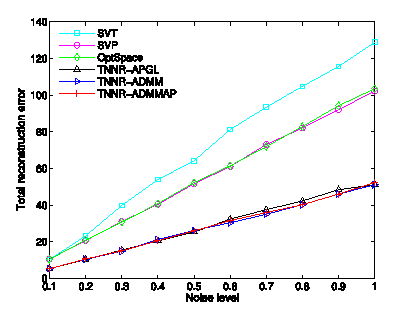
\includegraphics[width=0.45\textwidth]{./assets/ori-fig2-60.eps}}\quad\quad
    \subfloat[$70 \%$ observed]{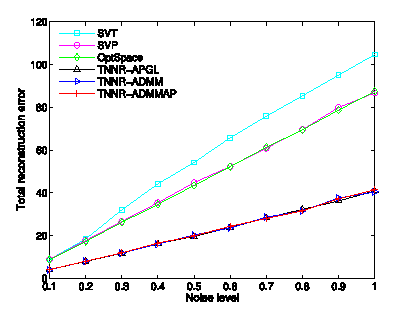
\includegraphics[width=0.45\textwidth]{./assets/ori-fig2-70.eps}}\\
    \subfloat[$80 \%$ observed]{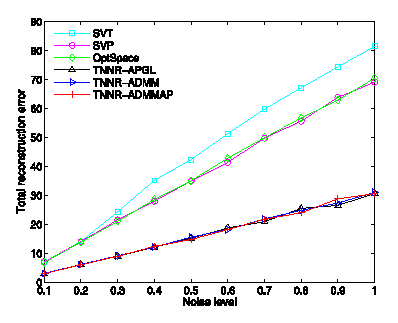
\includegraphics[width=0.45\textwidth]{./assets/ori-fig2-80.eps}}\quad\quad
    \subfloat[$90 \%$ observed]{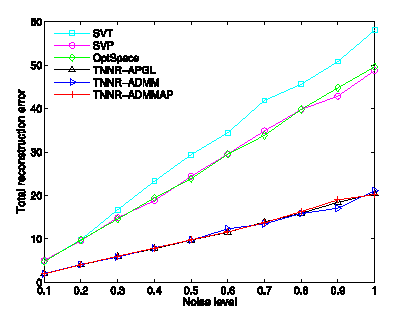
\includegraphics[width=0.45\textwidth]{./assets/ori-fig2-90.eps}}\\
    \caption{ The reconstruction error versus the noise level using the synthetic dataset. (The original result of paper)\label{fig2ori}}
\end{figure}
\begin{figure}[htbp]
    \centering
    \subfloat[$60 \%$ observed]{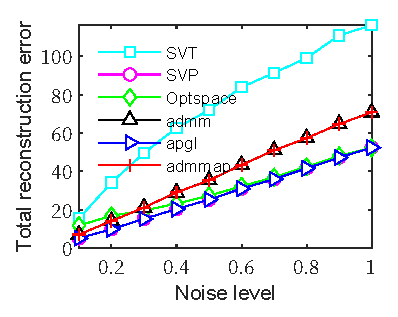
\includegraphics[width=0.45\textwidth]{./assets/fig2-60.eps}}\quad\quad
    \subfloat[$70 \%$ observed]{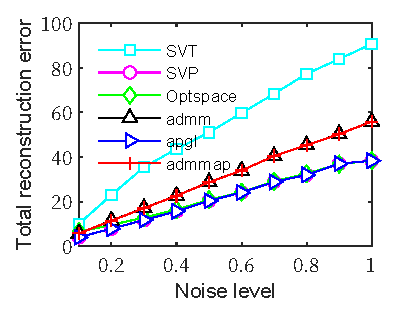
\includegraphics[width=0.45\textwidth]{./assets/fig2-70.eps}}\\
    \subfloat[$80 \%$ observed]{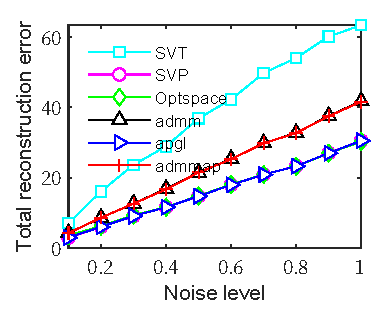
\includegraphics[width=0.45\textwidth]{./assets/fig2-80.eps}}\quad\quad
    \subfloat[$90 \%$ observed]{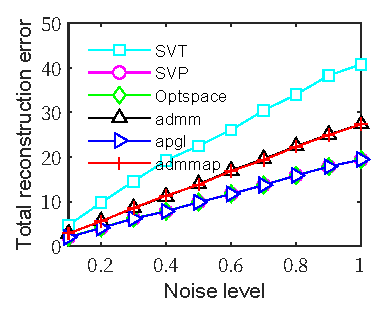
\includegraphics[width=0.45\textwidth]{./assets/fig2-90.eps}}\\
    \caption{ The reconstruction error versus the noise level using the synthetic dataset. (The results we reproduced)\label{fig2}}
\end{figure}

\begin{figure}[htbp]
    \centering
    \subfloat[$60 \%$ observed]{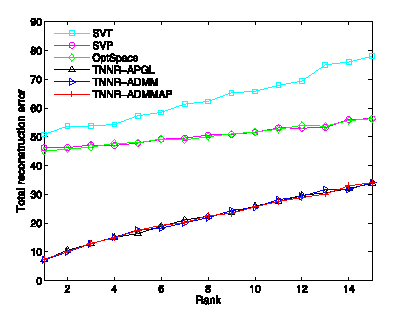
\includegraphics[width=0.45\textwidth]{./assets/ori-fig3-60.eps}}\quad\quad
    \subfloat[$70 \%$ observed]{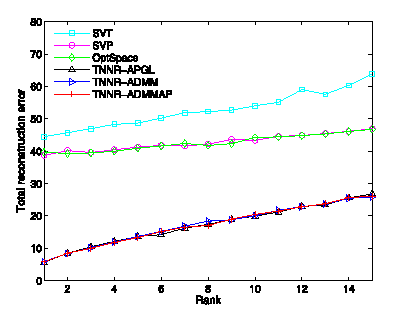
\includegraphics[width=0.45\textwidth]{./assets/ori-fig3-70.eps}}\\
    \subfloat[$80 \%$ observed]{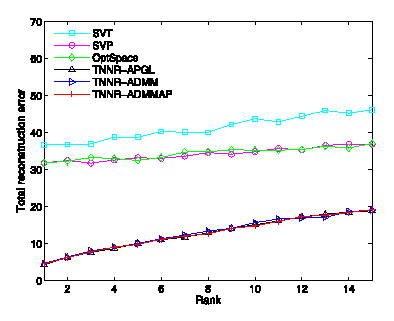
\includegraphics[width=0.45\textwidth]{./assets/ori-fig3-80.eps}}\quad\quad
    \subfloat[$90 \%$ observed]{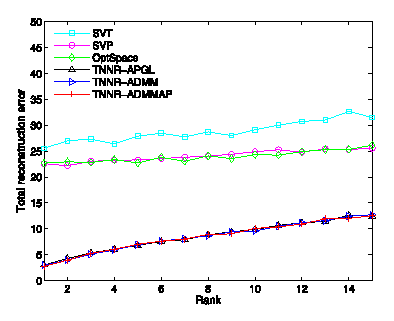
\includegraphics[width=0.45\textwidth]{./assets/ori-fig3-90.eps}}\\
    \caption{Recovery of an incomplete image with random mask. (The original result of paper)\label{fig3ori}}
\end{figure}
\begin{figure}[htbp]
    \centering
    \subfloat[$60 \%$ observed]{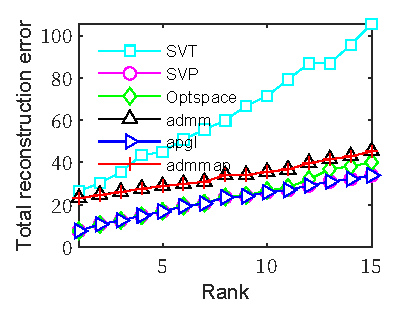
\includegraphics[width=0.45\textwidth]{./assets/fig3-60.eps}}\quad\quad
    \subfloat[$70 \%$ observed]{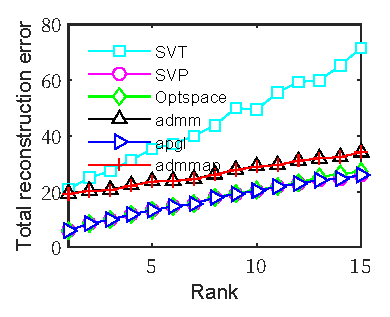
\includegraphics[width=0.45\textwidth]{./assets/fig3-70.eps}}\\
    \subfloat[$80 \%$ observed]{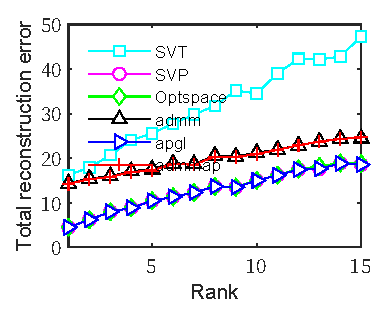
\includegraphics[width=0.45\textwidth]{./assets/fig3-80.eps}}\quad\quad
    \subfloat[$90 \%$ observed]{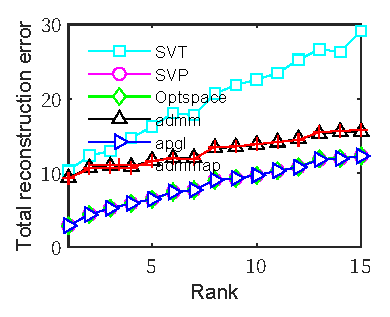
\includegraphics[width=0.45\textwidth]{./assets/fig3-90.eps}}\\
    \caption{ Recovery of an incomplete image with random mask. (The results we reproduced)\label{fig3}}
\end{figure}

As shown in Fig.~\ref{fig2}, under different noise levels and different observed ratios, compared with the original image:
\begin{itemize}
    \item Our reproduced (abbreviated as our)SVT algorithm has better overall reconstruction error performance.
    
    \item Our SVP and OptSpace performs better and has similar performance to TNNR-APGL.
    
    \item Our TNNR-ADMM performs similarly to the original image only at low noise levels. However, as the noise level increases, the performance deteriorates faster.
    
    \item Our TNNR-APGL has a similar performance to the original image.
\end{itemize}

As shown in Fig.~\ref{fig3}, under different observed ratios, as the
matrix rank increases, the total reconstruction error becomes larger. Compared with the original image:
\begin{itemize}
    \item Our SVT algorithm has better overall reconstruction error performance at low ranks, and our implementation of the SVT algorithm deteriorates more rapidly as the matrix rank increases.
    
    \item Our SVP and OptSpace performs better and has similar performance to TNNR-APGL.
    
    \item The total reconstruction error of our TNNR-ADMM and TNNR-ADMMAP is relatively large, and the results that are not close to the original work have been reached.
    
    \item Our TNNR-APGL has a similar performance to the original image.
\end{itemize}


\subsubsection{Parameter setting}
In our experiments, we readjusted the parameters of the six algorithms since the parameters given by the original author are incomplete and can not obtain good experimental results. Table~\ref{t1} shows the parameters set by the original author and us.

%\begin{table}
%	\caption{The parameters set in the paper}
%	\label{t1}
%	\centering
%	\renewcommand{\arraystretch}{1.25} 
%	\begin{tabular}{cccccccc}
%		\toprule
%		$\beta$  &$\lambda$ &$\beta_{max}$ & $\kappa$& $\rho_0$&$\epsilon_0$ & $\epsilon$  & $rank$\\
%		\midrule
%		$10^{-3}$ & $ 0.06 $ &  $10^{10}$ & $10^{-3}$ & $1.9$  & $10^{-3}$ & $10^{-4}$ & $1\sim 20$  \\
%		\bottomrule
%	\end{tabular}
%\end{table}

%
%\begin{table}
%	\caption{The parameters set in the paper}
%	\label{t1}
%	\centering
%	\renewcommand{\arraystretch}{1.25} 
%	\begin{tabular}{cc}
%		\toprule
%		parameter & value \\
%		\midrule
%		$\beta$  & $10^{-3}$   \\
%%		\hline
%		$\lambda$ & $ 0.06 $ \\
%%		\hline
%%		\cline{2-3}
%		 $\beta_{max}$ & $10^{10}$ \\
%%		\cline{2-3}
%		$\kappa$ & $10^{-3}$ \\
%%		\cline{2-3}
%		$\rho_0$ & $1.9$ \\
%%		\hline
%		 $\epsilon_0$ & $10^{-3}$ \\
%%		\hline
%		 $\epsilon$ & $10^{-4}$ \\
%%		\hline
%		$r$ & $1\sim 20$  \\
%		\bottomrule
%	\end{tabular}
%\end{table}

%\begin{table}
%	\caption{The parameters set in the paper}
%	\label{t1}
%	\centering
%	\renewcommand{\arraystretch}{1.25} 
%	\begin{tabular}{ccc}
%		\toprule
%		TNNR-ADMM & $\beta$  & $10^{-3}$   \\
%		\hline
%		TNNR-APGL & $\lambda$ & $ 0.06 $ \\
%		\hline
%		\multirow{4}{*}{TNNR-ADMMAP} & $\beta$ &  $10^{-3}$  \\
%		\cline{2-3}
%		& $\beta_{max}$ & $10^{10}$ \\
%		\cline{2-3}
%		& $\kappa$ & $10^{-3}$ \\
%		\cline{2-3}
%		& $\rho_0$ & $1.9$ \\
%		\hline
%		Algorithm~\ref{algo1} & $\epsilon_0$ & $10^{-3}$ \\
%		\hline
%		Algorithm~\ref{algo2}-\ref{algo4} & $\epsilon$ & $10^{-4}$ \\
%		\hline
%		Iteration rank & $r$ & $1\sim 20$  \\
%		\bottomrule
%	\end{tabular}
%\end{table}

%\begin{table}
%	\caption{The parameters we set}
%	\label{t2}
%	\centering
%	\renewcommand{\arraystretch}{1.25} 
%	\begin{tabular}{cccc}
%		\toprule
%		 Parameter  & Random mask & Text mask  & Block mask \\
%		\midrule
%		$p$ & 0.87 & 0.8 & 0.8 \\
%		%		\hline
%		$\delta_{2k}$ & 0.2 & 0.2 & 0.2 \\ 
%		%		\hline
%		 $\tau$ & $10^{-3}$ & $10^{-3}$ & $10^{-2}$ \\
%		%		\hline
%		 $\beta$  & $10^{-3}$  & $10^{-3}$ & $10^{-3}$\\
%		%		\hline
%		 $\lambda$ & $ 10^{-2} $ & $10^{-3}$ & $10^{-3}$ \\
%		%		\hline
%%		 $\beta$ &  $10^{-3}$ & $10^{-3}$ & $10^{-3}$\\
%		%		\cline{2-5}
%		$\beta_{max}$ & $10^{10}$ & $10^{10}$ & $10^{10}$ \\
%		%		\cline{2-5}
%		$\kappa$ & $10^{-3}$ & $10^{-3}$ & $10^{-3}$\\
%		%		\cline{2-5}
%		$\rho_0$ & $1.1$ & $1.01$ & $1.01$\\
%		%		\hline
%		 $\epsilon_0$ & $10^{-3}$ & $10^{-3}$ & $10^{-3}$\\
%		%		\hline
%		 $\epsilon$ & $10^{-4}$ & $10^{-4}$ & $10^{-4}$\\
%		%		\hline
%		$rank$ & $5$ & $3\sim 20$ & $3$ \\
%		%		\hline
%		 $iter_{max}$ & $10^2$ & $10^2/10^3$ & $10^2/10^3$ \\
%		\bottomrule
%	\end{tabular}
%\end{table}

\begin{table}
	\caption{The parameters set by the original author and us}
	\label{t1}
	\centering
	\renewcommand{\arraystretch}{1.25} 
	\begin{tabular}{ccccc}
		\toprule
		Parameter  & Random mask & Text mask  & Block mask & Paper set\\
		\midrule
		$p$ & 0.87 & 0.8 & 0.8 & \\
		%		\hline
		$\delta_{2k}$ & 0.2 & 0.2 & 0.2 & \\ 
		%		\hline
		$\tau$ & $10^{-3}$ & $10^{-3}$ & $10^{-2}$ & \\
		%		\hline
		$\beta$  & $10^{-3}$  & $10^{-3}$ & $10^{-3}$ & $10^{-3}$\\
		%		\hline
		$\lambda$ & $ 10^{-2} $ & $10^{-3}$ & $10^{-3}$ & $0.06$\\
		%		\hline
		%		 $\beta$ &  $10^{-3}$ & $10^{-3}$ & $10^{-3}$\\
		%		\cline{2-5}
		$\beta_{max}$ & $10^{10}$ & $10^{10}$ & $10^{10}$ & $10^{10}$\\
		%		\cline{2-5}
		$\kappa$ & $10^{-3}$ & $10^{-3}$ & $10^{-3}$ & $10^{-3}$\\
		%		\cline{2-5}
		$\rho_0$ & $1.1$ & $1.01$ & $1.01$ & $1.9$\\
		%		\hline
		$\epsilon_0$ & $10^{-3}$ & $10^{-3}$ & $10^{-3}$ & $10^{-3}$\\
		%		\hline
		$\epsilon$ & $10^{-4}$ & $10^{-4}$ & $10^{-4}$ & $10^{-4}$\\
		%		\hline
		$rank$ & $5$ & $3\sim 20$ & $3$ & $1\sim 20$\\
		%		\hline
		$iter_{max}$ & $10^2$ & $10^2/10^3$ & $10^2/10^3$ & \\
		\bottomrule
	\end{tabular}
\end{table}

\subsubsection{Random mask}
\label{random}
we randomly cover some pixels of an image ($300 \times 300$), and then compare the recovery performance of the six algorithms.The results are shown in Fig.~\ref{fig4} and Fig.~\ref{fig5}. Naturally, the larger the observed ratio is the better recovery of the image that can be achieved. Form Fig.~\ref{fig5}, we can see that the TNNR-based algorithms can achieve higher PSNR values compared with the other three methods. Compare with the results in the original paper, our SVT recovers images better. And the results of TNNR-APGL are not as expected in the high observed ratio.

\begin{figure}[htbp]
	\centering
	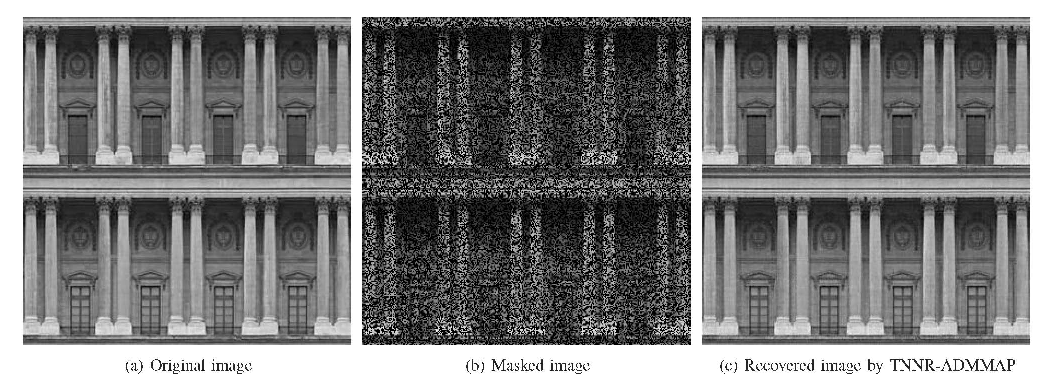
\includegraphics[width=1\textwidth]{./assets/ori-fig4.eps}
	\caption{The reconstruction error versus the matrix rank ($r_0$) using the synthetic dataset. (The original result of paper)}
	\label{fig4ori}
\end{figure}
\begin{figure}[htbp]
	\centering
	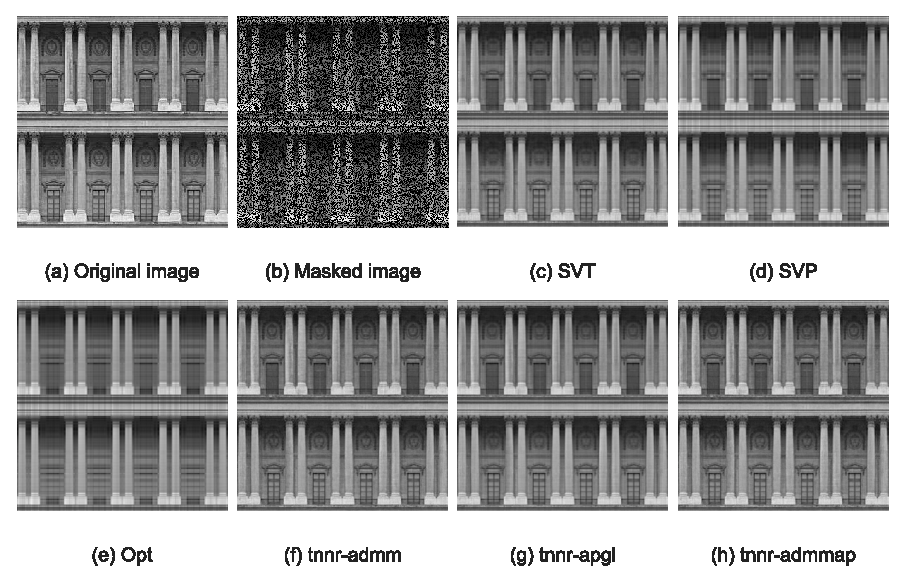
\includegraphics[width=1\textwidth]{./assets/fig4.eps}
	\caption{The reconstruction error versus the matrix rank ($r_0$) using the synthetic dataset. (The result we reproduced)}
	\label{fig4}
\end{figure}

\begin{figure}[htbp]
	\centering
	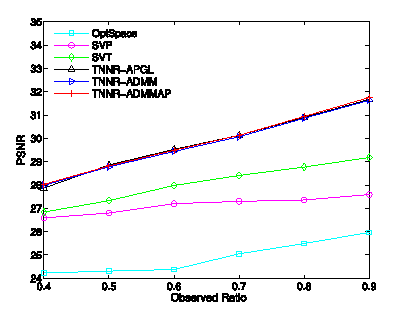
\includegraphics[width=0.6\textwidth]{./assets/ori-fig5.eps}
	\caption{The PSNR values of the recovered image under different
		observed ratios (random mask) by all six methods. (The original result of paper)}
	\label{fig5ori}
\end{figure}
\begin{figure}[htbp]
	\centering
	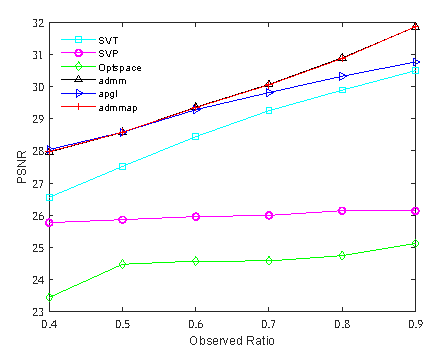
\includegraphics[width=0.6\textwidth]{./assets/fig5.eps}
	\caption{The PSNR values of the recovered image under different
		observed ratios (random mask) by all six methods. (The result we reproduced)}
	\label{fig5}
\end{figure}

\begin{figure}[htbp]
	\centering
	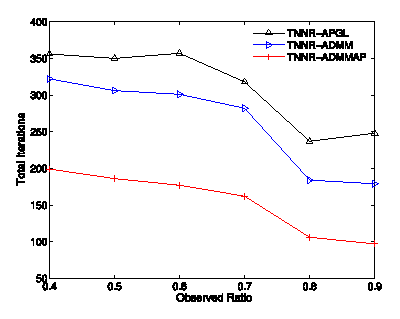
\includegraphics[width=0.6\textwidth]{./assets/ori-fig6.eps}
	\caption{Iterations needed for our three TNNR-based algorithms to recover the given
		randomly masked image under different observed ratios. (The original result of paper)}
	\label{fig6ori}
\end{figure}
\begin{figure}[htbp]
	\centering
	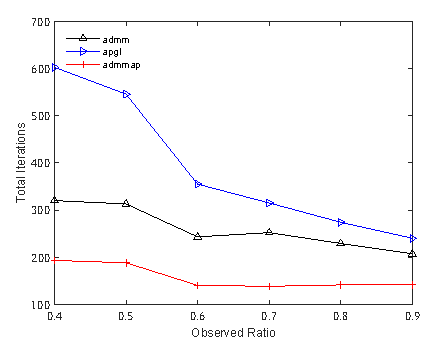
\includegraphics[width=0.6\textwidth]{./assets/fig6.eps}
	\caption{Iterations needed for our three TNNR-based algorithms to recover the given
		randomly masked image under different observed ratios. (The result we reproduced)}
	\label{fig6}
\end{figure}

\subsubsection{Text mask}
\label{text}

Since the text is not random, it may cover important information in the picture, making the text more difficult to remove than pixels. Fig.~\ref{fig7} and Fig.~\ref{fig8} show the experimental results of the six matrix
completion algorithms. Specifically, for the example image
in Fig.~\ref{fig7}, the PSNR values for SVT, SVP, OptSpace, TNNR-
ADMM, TNNR-APGL, and TNNR-ADMMAP are 23.47,
23.47, 22.43, 25.26, 25.26, and 25.27, respectively. And for the
example image in Fig.~\ref{fig8}, the PSNR values for SVT, SVP,
OptSpace, TNNR-ADMM, TNNR-APGL, and TNNR-ADMMAP are 21.61, 21.61, 21.95, 23.94, 23.16, and 23.95, respectively. 
From these results we can see that TNNR-ADMM and TNNR-ADMMAP algorithms achieve better performance than the other three matrix completion algorithms. Our TNNR-APGL cannot obtain the same image restoration effect as the original paper.

\begin{figure}[htbp]
	\centering
	\includegraphics[width=1\textwidth]{./assets/fig7.eps}
	\caption{Comparison of matrix completion algorithms for text removal problem. (The original result of paper)}
	\label{fig7ori}
\end{figure}
\begin{figure}[htbp]
	\centering
	\includegraphics[width=1\textwidth]{./assets/fig7.eps}
	\caption{Comparison of matrix completion algorithms for text removal problem. (The result we reproduced)}
	\label{fig7}
\end{figure}

\begin{figure}[htbp]
	\centering
	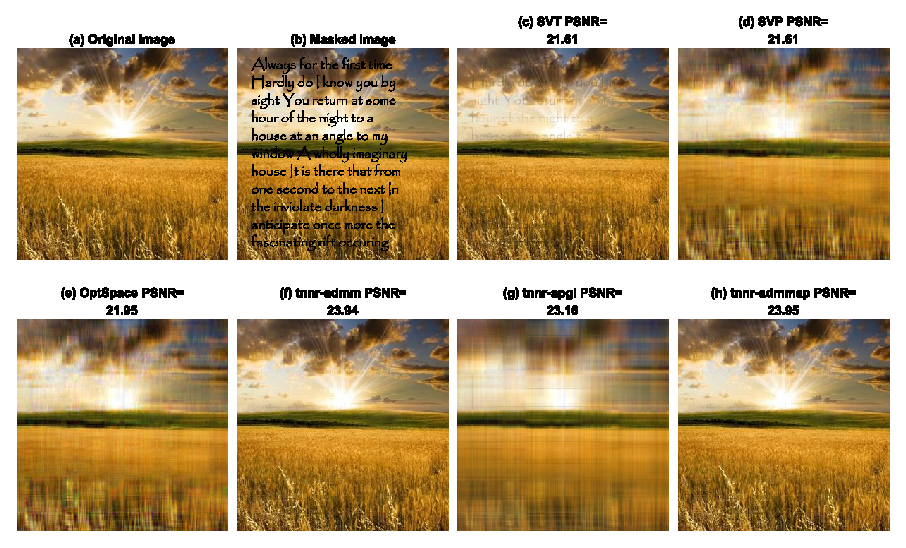
\includegraphics[width=1\textwidth]{./assets/fig8.eps}
	\caption{Comparison of matrix completion algorithms for text removal problem. (The original result of paper)}
	\label{fig8ori}
\end{figure}
\begin{figure}[htbp]
	\centering
	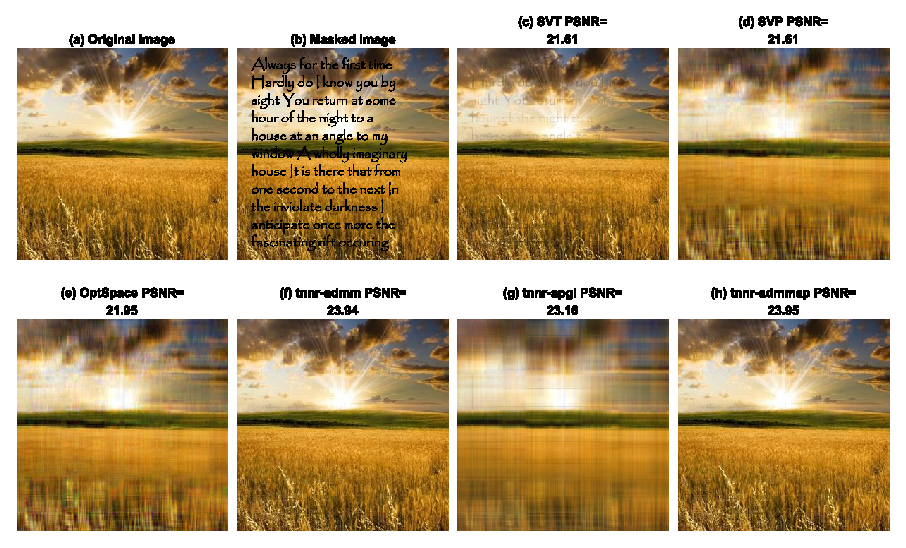
\includegraphics[width=1\textwidth]{./assets/fig8.eps}
	\caption{Comparison of matrix completion algorithms for text removal problem. (The result we reproduced)}
	\label{fig8}
\end{figure}


\subsubsection{Block mask}
In some situations, Some pixels in the image have been broken. We first mask all these pixels, then we use six matrix completion algorithms to recover these large missing blocks.
Fig.~\ref{fig9} show the recovered images by using the six different matrix completion algorithms.
Similar to the text mask, our TNNR-ADMM and TNNR-ADMMAP can recover the image better, but the the image recovered by our TNNR-APGl loses a lot of texture information.
\begin{figure}[htbp]
	\centering
	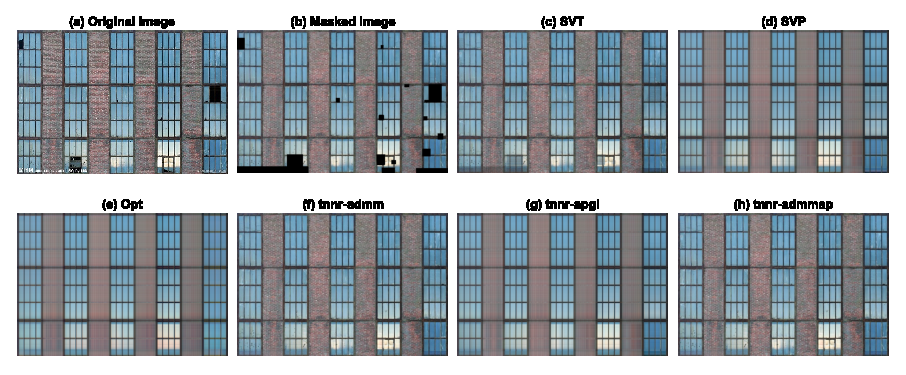
\includegraphics[width=1\textwidth]{./assets/fig9.eps}
	\caption{Comparison of different methods for recovering missing blocks of
		a natural image. (The original result of paper)}
	\label{fig9ori}
\end{figure}
\begin{figure}[htbp]
	\centering
	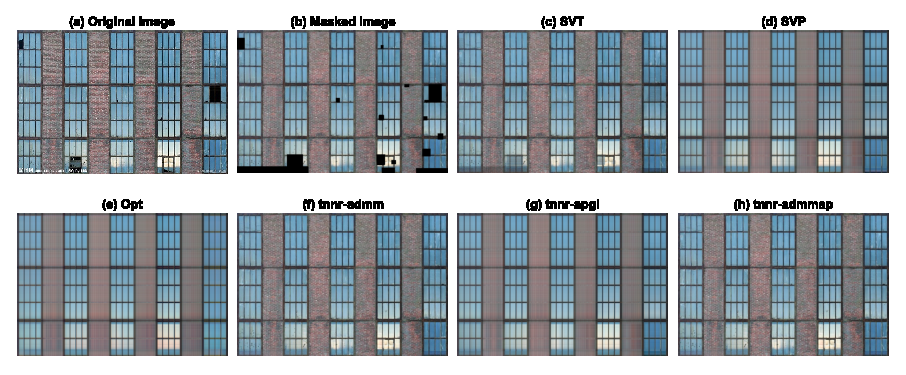
\includegraphics[width=1\textwidth]{./assets/fig9.eps}
	\caption{Comparison of different methods for recovering missing blocks of
		a natural image. (The result we reproduced)}
	\label{fig9}
\end{figure}

\subsection{Convergence rate and computational cost}
In the experiments in Fig.~\ref{fig4}, we also tested the total number of iterations for the TNNR algorithm to recover images under different observed ratios. First, from Fig.~\ref{fig5}, we observe that in low observed ratio, the three TNNR-based algorithms have close PSNR again, while in high observed ratio, TNNR-APGL has lower PSNR. As shown in Fig.~\ref{fig6}, TNNR-ADMMAP converges much faster than TNNR-APGL and TNNR-ADMM. The total number of iterations needed for TNNR-ADMMAP to converge is roughly half of that for TNNR-APGL and TNNR-ADMM, while They obtain almost the same result. 

Considering that the time cost of each iteration of the three algorithms is slightly different, in the text mask experiment, we tested the total time required for the six algorithms to recover the image, and the rank of the best PSNR , as shown in the Table~\ref{t3}. The time required for SVT is the shortest. Among the three TNNR-based algorithms, TNNR-ADMM takes the shortest time, and TNNR-APGL takes the longest time. Different from the original work, our implementation of the TNNR-ADMMAP algorithm does not show the convergence speed of the original paper, which is slower than the TNNR-ADMM algorithm, but faster than TNNR-APGL.

\begin{table}
	\caption{The total time required for the six algorithms in text mask experiment}
	\label{t3}
	\centering
	\renewcommand{\arraystretch}{1.25} 
	\begin{tabular}{ccccc}
		\toprule
		\multirow{2}{*}{Algorithm}  & \multicolumn{2}{c}{Fig.~\ref{fig7}} & \multicolumn{2}{c}{Fig.~\ref{fig8}} \\
		\cmidrule(r){2-3} \cmidrule(r){4-5} 
		& Total time (s) & Best rank & Total time (s) & Best rank \\
		\midrule
		SVT & $60.410$ & no need &   $25.128$ &  no need \\
%		\hline
		SVP & $1856.893$ & $15$ & $253.012$ & $11$ \\
%		\hline
		OptSpace & $1856.893$ & $15$ & $253.012$ & $13$ \\
%		\hline
		TNNR-ADMM &  $371.048$ & $15$ & $314.183$ & $6$\\
%		\hline
		TNNR-APGL & $1175.097$ & $3$ & $1509.657$ & $3$\\
%		\hline
		TNNR-ADMMAP & $759.241$ & $15$ & $570.614$ & $6$\\
 		\bottomrule
	\end{tabular}
\end{table}

\section{Conclusion}
\label{s5}
In this report, we replicate the paper by Yao Hu et al. This paper proposes a new matrix completion method called truncated nuclear
norm regularization. This approach tries to minimize the summation of the smallest $\min (m,n)-r$ singular values, where $r$ is the matrix rank. 
Moreover, they also designed a two-step iterative solution, and performed three optimizations based on ADMM, APGL, and ADMMAP for the second iteration. We conduct similar experiments on synthetic and real visual datasets and compare with the original results. The experimental results demonstrate the advantages of the TNNR-based algorithms in comparison with
three matrix completion methods based on the nuclear norm or matrix factorization. However, there are some differences between our reproduction results and the results shown in the author's paper. Because the author's parameters cannot play well in this reproduction, the reason may be that our parameters are not adjusted to the best, or the author may have preprocessed the image.



%\section*{References}

\medskip
{\small{}\bibliographystyle{unsrt}
\bibliography{report}
}{\small\par}

%%%%%%%%%%%%%%%%%%%%%%%%%%%%%%%%%%%%%%%%%%%%%%%%%%%%%%%%%%%%



\appendix


\section{Appendix}
\textit{proof} Theorem~\ref{thm31}

By Von Neumann's trace inequality, we get
\begin{equation}
    \begin{aligned}
        \text{Tr}(\mathbf A\mathbf X\mathbf B^T) & = \text{Tr}(\mathbf X\mathbf B^T\mathbf A) \\
        & \leq  \sum_{i=1}^{\min(m,n)} \sigma_i(\mathbf X) \sigma_i(\mathbf B^T\mathbf A),
    \end{aligned}
\end{equation}
where $\sigma_1(\mathbf X) \geq \cdots \geq \sigma_{min(m,n)}(\mathbf X) \geq 0 $. As $\text{rank}(\mathbf A) = r$ and $\text{rank}(\mathbf B) =r$, so $\text{rank}(\mathbf B^T\mathbf A) =s \leq r$. For $i \leq s$, $\sigma_i(\mathbf B^T\mathbf A) \geq 0$ and $\sigma_i(\mathbf B^T\mathbf A)$ is the $i$th eigenvalue of $\mathbf B\mathbf B^T=I$. Therefore, $\sigma_i(\mathbf B^T\mathbf A) = 1$, for $i=1,2,\dots,s$, and the rest are all 0s. It follows that:
\begin{equation}
    \begin{aligned}
        \sum_{i=1}^{\min(m,n)} \sigma_i(\mathbf X) \sigma_i(\mathbf B^T\mathbf A) & = \sum_{i=1}^{s} \sigma_i(\mathbf X) \sigma_i(\mathbf B^T\mathbf A) + \sum_{i=s+1}^{\min(m,n)} \sigma_i(\mathbf X) \sigma_i(\mathbf B^T\mathbf A) \\
        & = \sum_{i=1}^{s} \sigma_i(\mathbf X) \cdot 1 + \sum_{i=s+1}^{\min(m,n)} \sigma_i(\mathbf X) \cdot 0 \\
        & = \sum_{i=1}^{s} \sigma_i(\mathbf X).
    \end{aligned}
\end{equation}
Since $s \leq r$ and $\sigma_i(\mathbf X) \geq 0$:
\begin{equation*}
    \sum_{i=1}^s \sigma_i(\mathbf X)\leq \sum_{i=1}^r \sigma_i(\mathbf X).
\end{equation*}
Combining inequalities and ,we have 
\begin{equation}
    \text{Tr}(\mathbf A\mathbf X\mathbf B^T) \leq \sum_{i=1}^s \sigma_i(\mathbf X)\leq \sum_{i=1}^r \sigma_i(\mathbf X).
\end{equation}


\textit{proof} Equation~\ref{admmx}

Fix $\mathbf W_k$ and $\mathbf Y_k$ ,
\begin{equation}
    \mathbf X_{k+1} =  \underset{\mathbf X}{\arg\min} \ \Vert\mathbf X \Vert_* - \text{Tr}(\mathbf A_l \mathbf W_k\mathbf B_l^T)    + \frac{\beta}{2}\Vert\mathbf X-\mathbf W_k \Vert_F^2 + \text{Tr}(\mathbf Y_k(\mathbf X-\mathbf W_k)).
    \label{xeq1}
\end{equation}
For the last two terms of \eqref{xeq1},
\begin{equation}
\frac{\beta}{2}\Vert\mathbf X-\mathbf W_k \Vert_F^2 + \text{Tr}(\mathbf Y_k^T(\mathbf X-\mathbf W_k))=  \frac{\beta}{2}\left( \Vert\mathbf X-\mathbf W_k \Vert_F^2 + \frac{2}{\beta} \text{Tr}(\mathbf Y_k^T(\mathbf X-\mathbf W_k)) \right).
\label{xeq2}
\end{equation}
Because
\begin{equation*}
    \begin{aligned}
        \Vert\mathbf X-\mathbf W_k+\frac{1}{\beta}\mathbf Y_k \Vert_F^2 & = \text{Tr} \ (\mathbf X-\mathbf W_k+\frac{1}{\beta}\mathbf Y_k)(\mathbf X-\mathbf W_k+\frac{1}{\beta}\mathbf Y_k)^T \\
        & = \text{Tr}(\mathbf X-\mathbf W_k)(\mathbf X-\mathbf W_k)^T + 2\ \text{Tr}(\mathbf X-\mathbf W_k)\frac{1}{\beta}\mathbf Y_k^T + \frac{1}{\beta^2}\text{Tr} (\mathbf Y_k Y_k^T) \\
        & = \Vert\mathbf X-\mathbf W_k \Vert_F^2 + \frac{1}{\beta^2}\Vert\mathbf Y_k \Vert_F^2 + \frac{2}{\beta}\text{Tr}(\mathbf Y_k^T(\mathbf X-\mathbf W_k)).
    \end{aligned}
\end{equation*}
For the latter term in parentheses of \eqref{xeq2},
\begin{equation}
    \begin{aligned}
\frac{2}{\beta} \text{Tr}(\mathbf Y_k^T(\mathbf X-\mathbf W_k)) & =  2 \ \text{Tr}(\frac{1}{\beta}\mathbf Y_k^T(\mathbf X-\mathbf W_k)) \\
    & = \Vert\mathbf X-\mathbf W_k+\frac{1}{\beta}\mathbf Y_k \Vert_F^2 - \frac{1}{\beta^2}\Vert\mathbf Y_k \Vert_F^2 - \Vert\mathbf X-\mathbf W_k \Vert_F^2.
\end{aligned}
\end{equation}
Ignoring all constant terms, 
\begin{equation}
\begin{aligned}
    \mathbf X_{k+1} & =\underset{\mathbf X}{\arg\min}\ L(\mathbf X,\mathbf Y_k, \mathbf W_k,\beta) \\
    & =  \underset{\mathbf X}{\arg\min} \ \Vert\mathbf X \Vert_* - \text{Tr}(\mathbf A_l\mathbf W_k\mathbf B_l^T)    + \frac{\beta}{2}\Vert\mathbf X-\mathbf W_k \Vert_F^2 + \text{Tr}(\mathbf Y_k^T(\mathbf X-\mathbf W_k)) \\
    & = \underset{\mathbf X}{\arg\min} \ \Vert\mathbf X \Vert_* + \frac{\beta}{2} \Vert\mathbf X-\left(\mathbf W_k - \frac{1}{\beta}\mathbf Y_k \right) \Vert_F^2 - \frac{1}{2\beta} \Vert\mathbf Y_k \Vert_F^2 \\
    & = \underset{\mathbf X}{\arg\min} \ \Vert\mathbf X \Vert_* + \frac{\beta}{2} \Vert\mathbf X-\left(\mathbf W_k - \frac{1}{\beta}\mathbf Y_k \right) \Vert_F^2.
\end{aligned} 
\end{equation}
That is 
\begin{equation}
    \mathbf X_{k+1} = D_{\frac{1}{\rho}}(\mathbf W_k - \frac{1}{\rho}\mathbf Y_k).
\end{equation}

\end{document}